\clearpage
\section{New Developments: Refraction Map and Extended Refraction Experiments}
\label{sec:new-developments}

\subsection{Derivation of the smooth refraction map}

\subsubsection{Step 1: Write the refractor as an implicit surface}

Starting with the softmin potential,
\begin{align}
 f_\varepsilon(x)
 &=-\varepsilon\log\sum_jq_j
   \exp\!\left(\frac{g_j-c_\kappa(x,y_j)}{\varepsilon}\right),
 \\
 c_\kappa(x,y_j)&=-\log(1-\kappa x\cdot y_j),
\end{align}
the refractor radius is
\begin{equation}
 R(x)=e^{f_\varepsilon(x)}
 =\left[\sum_jq_je^{g_j/\varepsilon}
           (1-\kappa x\cdot y_j)^{1/\varepsilon}\right]^{-\varepsilon}.
\end{equation}
Write $a_j=q_je^{g_j/\varepsilon}$. Raising both sides to the power
$-1/\varepsilon$ gives
\[
 R(x)^{-1/\varepsilon}
 =\sum_j a_j(1-\kappa x\cdot y_j)^{1/\varepsilon}.
\]
Multiplying by $R(x)^{1/\varepsilon}$ yields
\[
 \sum_j a_j[R(x)(1-\kappa x\cdot y_j)]^{1/\varepsilon}=1.
\]
Since $p=R(x)x$ and $\|p\|=R(x)$,
\[
 R(x)(1-\kappa x\cdot y_j)=\|p\|-\kappa p\cdot y_j.
\]
Therefore the refractor satisfies
\begin{equation}
 \boxed{F(p)=\sum_j a_j(\|p\|-\kappa p\cdot y_j)^{1/\varepsilon}-1=0.}
 \label{eq:new-implicit-refractor}
\end{equation}

\subsubsection{Step 2: Take the ordinary gradient to obtain a normal}

Using the gradient identities,
\[
 \nabla_p\|p\|=\frac{p}{\|p\|},
 \qquad \nabla_p(\kappa p\cdot y_j)=\kappa y_j.
\]
The chain rule gives
\begin{equation}
 \nabla F(p)=\frac1\varepsilon\sum_j
 a_j(\|p\|-\kappa p\cdot y_j)^{1/\varepsilon-1}
 \left(\frac{p}{\|p\|}-\kappa y_j\right).
\end{equation}
At the surface point $p=R(x)x$, abbreviate $R=R(x)$ and
$d_j(x)=1-\kappa x\cdot y_j$. Then
\begin{align}
 \nabla F(Rx)
 &=\frac1\varepsilon\sum_j a_j(Rd_j)^{1/\varepsilon-1}
       (x-\kappa y_j) \\
 &=\frac1{\varepsilon R}\sum_j
       a_j(Rd_j)^{1/\varepsilon}\frac{x-\kappa y_j}{d_j}.
 \label{eq:new-gradient-at-radius}
\end{align}
The second line uses
$(Rd_j)^{1/\varepsilon-1}=(Rd_j)^{1/\varepsilon}/(Rd_j)$.
We now explain exactly how its coefficients become the weights $w_j(x)$.

\paragraph{What is $w_j(x)$?}
Define the positive normalizing sum
\[
 Z(x)=\sum_k q_ke^{g_k/\varepsilon}
                  (1-\kappa x\cdot y_k)^{1/\varepsilon}
     =\sum_k a_kd_k(x)^{1/\varepsilon}.
\]
The radius formula says $R(x)=Z(x)^{-\varepsilon}$, so
\[
 R(x)^{1/\varepsilon}=Z(x)^{-1}.
\]
Consequently, each coefficient in
\eqref{eq:new-gradient-at-radius} satisfies
\begin{align}
 a_j[R(x)d_j(x)]^{1/\varepsilon}
 &=a_jR(x)^{1/\varepsilon}d_j(x)^{1/\varepsilon} \\
 &=\frac{a_jd_j(x)^{1/\varepsilon}}{Z(x)} \\
 &=\frac{q_je^{g_j/\varepsilon}
              (1-\kappa x\cdot y_j)^{1/\varepsilon}}
         {\sum_kq_ke^{g_k/\varepsilon}
              (1-\kappa x\cdot y_k)^{1/\varepsilon}} \\
 &=:w_j(x).
 \label{eq:new-softmin-weights}
\end{align}
Equivalently, in the original softmin notation,
\begin{equation}
 w_j(x)=
 \frac{q_j\exp((g_j-c_\kappa(x,y_j))/\varepsilon)}
      {\sum_kq_k\exp((g_k-c_\kappa(x,y_k))/\varepsilon)}.
\end{equation}
Thus $w_j(x)$ is the normalized contribution of target direction $y_j$
to the softmin at $x$: $w_j(x)\geq0$ and $\sum_jw_j(x)=1$.
These local, $x$-dependent weights differ from the prescribed target
masses $q_j$.

Substituting these weights into the gradient gives
\[
 \nabla F(Rx)=\frac1{\varepsilon R}N_\kappa(x),
\]
where the unnormalized normal is
\begin{equation}
 \boxed{N_\kappa(x)=\sum_jw_j(x)
              \frac{x-\kappa y_j}{1-\kappa x\cdot y_j}.}
 \label{eq:new-normal}
\end{equation}
Multiplication by $1/(\varepsilon R)>0$ does not change its direction.
Moreover,
\begin{equation}
 x\cdot N_\kappa(x)
 =\sum_jw_j(x)\frac{1-\kappa x\cdot y_j}
                       {1-\kappa x\cdot y_j}
 =1.
 \label{eq:new-normal-identity}
\end{equation}
This identity remains $x\cdot N_\kappa=1$; the factors of $\kappa$ cancel
inside the sum. In particular, the normal is nonzero.

\subsection{Extended refraction experiments: common setup}

We completed experiments 1--3 twice: once with the inherited final-loop
limits of 17 transport updates and 17 updates per self solve, and once
with both limits raised to 2000. The target was held fixed at
\textbf{1600 points in every evaluation}; only the source point count
and refractor regularization were varied. Both runs use the same Halton
patches and normalized density weights described earlier, with
\[
 \kappa=0.6,\qquad
 \varepsilon_{\mathrm{eval}}=\frac1{320}=0.003125.
\]
The source count has 40 logarithmically spaced values, rounded to integers,
from 100 to 20,000. The refractor epsilon grid has 40 logarithmically
spaced values from $0.0000625$ to $0.025$.
\begin{enumerate}
 \item \textbf{Joint movement:} vary the source count $N_K$ and set
 $\varepsilon_{\mathrm{refr}}=1/(8\lfloor\sqrt{N_K}\rfloor)$.
 \item \textbf{Fixed refractor epsilon:} vary the source count $N_K$
 with $\varepsilon_{\mathrm{refr}}=1/320$.
 \item \textbf{Fixed source count:} fix $N_K=1600$ and vary
 $\varepsilon_{\mathrm{refr}}$ over the 40-value epsilon grid.
\end{enumerate}
Each experiment has 40 evaluations, giving 120 per run and 240 in total.
The refractor potential-change tolerance remains $10^{-5}$ in both runs;
the independent PF evaluation tolerance is $10^{-9}$. The small-grid and
continuation schedules were retained. Rectangular transports use each
marginal's own support for smoothing and self-cost corrections.

\paragraph{Clarification of the iteration count.}
The earlier notes used the internal variable \texttt{cap\_iter=16}.
The inherited loop checks $i>16$ \emph{after} an update, permitting
17 final updates. The comparable baseline is therefore labeled 17/17,
and the new run 2000/2000. These limits apply to the final loops;
warm-start and continuation updates are additional. The current solver
uses a small-grid warm start and continuation, rather than a cold start
directly at the final regularization.

\subsection{What the plotted cost measures}

The discrete push-forward in these experiments is the hard $c$-transform
map used by the existing refractor pipeline:
\[
 j^*(i)=\underset{j}{\operatorname{argmin}}
       \{c_\kappa(x_i,y_j)-g_j^{\mathrm{raw}}\},
 \qquad z_i=y_{j^*(i)},\qquad
 \alpha=\sum_i p_i\delta_{z_i},\quad
 \nu=\sum_{j=1}^{1600}q_j\delta_{y_j}.
\]
The plotted objective is the \emph{entropically regularized OT objective}
between this pushed measure and the prescribed target:
\begin{equation}
\begin{aligned}
 \operatorname{EOT}_{\eta}(\alpha,\nu)
 &=\min_{\pi\in\Pi(p,q)}
 \left\{\sum_{i,j}\pi_{ij}\|z_i-y_j\|_2^2
 +\eta\,\operatorname{KL}(\pi\mid p\otimes q)\right\},
 \\
 &\hspace{1cm}\eta=\frac1{320}.
\end{aligned}
 \label{eq:new-eot-evaluation}
\end{equation}
The ground cost is squared Euclidean distance between unit directions in
three-dimensional coordinates. In contrast to the earlier illustrative
error diagnostics, these plots show the EOT objective itself, without
self-term subtraction or a square root. They do not plot the optical
solver's approximate internal \texttt{total\_cost}. Keeping
$\varepsilon_{\mathrm{eval}}$ fixed separates the evaluation regularization
from the refractor epsilon being swept. A nonzero regularized objective
alone does not imply that the pushed and target measures differ.

\subsection{Completed results and marginal diagnostics}

Both runs contain 120 finite EOT values, with 40 distinct parameter pairs
per experiment and successful PF evaluation convergence for every row.
The grids, fixed target size, checkpoint names, and source/target array
lengths were checked. These checks establish completion of the numerical
evaluations; they do not establish exact marginal feasibility of the
underlying refractor transport.

For the refractor plan
\[
 \gamma_{ij}=p_iq_j
 \exp\!\left(\frac{f_i^{\mathrm{raw}}+g_j^{\mathrm{raw}}
                         -c_\kappa(x_i,y_j)}
                        {\varepsilon_{\mathrm{refr}}}\right),
\]
the reported source and target marginal residuals are
\[
 r_s=\sum_i\left|\sum_j\gamma_{ij}-p_i\right|,
 \qquad
 r_t=\sum_j\left|\sum_i\gamma_{ij}-q_j\right|.
\]
Their ranges across all 120 solves in each run are:
\begin{center}
\small
\resizebox{\textwidth}{!}{%
\begin{tabular}{lcc}
\hline
Transport / self cap & Source marginal $r_s$ & Target marginal $r_t$ \\
\hline
17 / 17 & $[2.5085\!\times\!10^{-7},\,0.17678]$
        & $[1.7388\!\times\!10^{-4},\,0.54792]$ \\
2000 / 2000 & $[5.2395\!\times\!10^{-9},\,0.014721]$
            & $[1.7388\!\times\!10^{-4},\,0.014721]$ \\
\hline
\end{tabular}
}
\end{center}
The maximum source residual decreases by about a factor of 12, and the
maximum target residual by about a factor of 37. The larger limits improve
the worst observed marginal errors but do not force them to zero.

In the 2000-cap run, all final loops met the $10^{-5}$ potential-change
tolerance before reaching their caps:
\begin{center}
\begin{tabular}{lrrr}
\hline
Final loop & Met tolerance & Hit cap & Most updates \\
\hline
Transport & 120 & 0 & 659 \\
Source self solve & 120 & 0 & 551 \\
Target self solve & 120 & 0 & 15 \\
\hline
\end{tabular}
\end{center}
Small potential changes, small marginal residuals, and convergence of the
separate EOT evaluation are three different diagnostics and should be
reported separately.

\subsection{Reading the three experiments}

In experiment 1, the 2000-cap EOT objective decreases from approximately
$0.0074033$ at $N_K=100$ to $0.0060977$ at $N_K=20000$.
The baseline ends at approximately $0.0066790$ and has a nonmonotone tail.
Experiment 2 varies only the source discretization and stays in the narrow
range $0.0063749$--$0.0064001$ for both runs; raising the caps does not
produce a large improvement in this objective.
In experiment 3, the two curves are close: the largest pointwise
difference in the saved EOT values is approximately $1.84\times10^{-5}$.
Both run from approximately $0.0059669$ at the smallest refractor epsilon
to $0.0084764$ at the largest. Similar hard-map objectives do not imply
similar underlying potentials or marginal residuals. These observations describe the tested grids,
rather than proving an asymptotic convergence rate.

\clearpage
\begin{figure}[p]
 \centering
 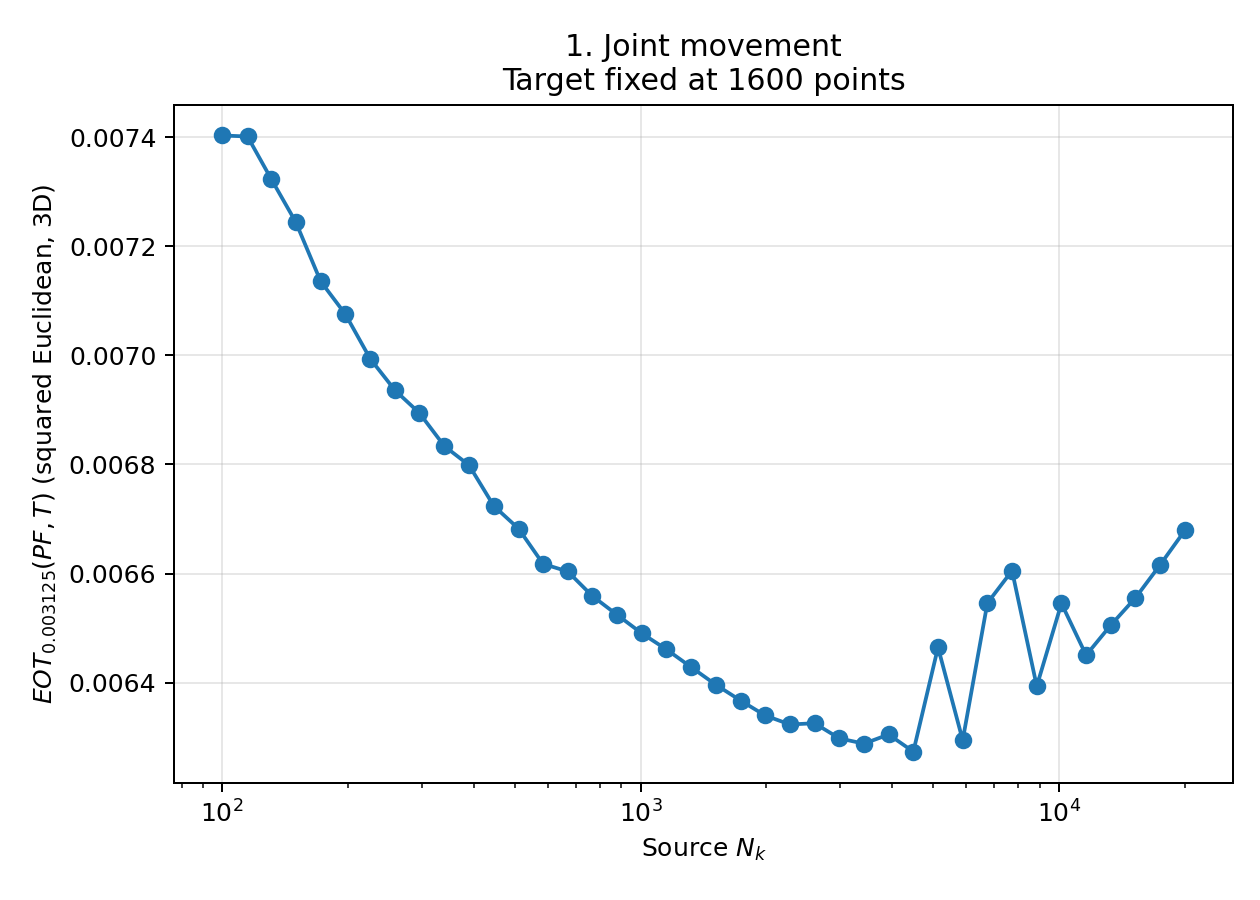
\includegraphics[width=0.88\textwidth]{baseline_experiment_1.png}
 \par\smallskip
 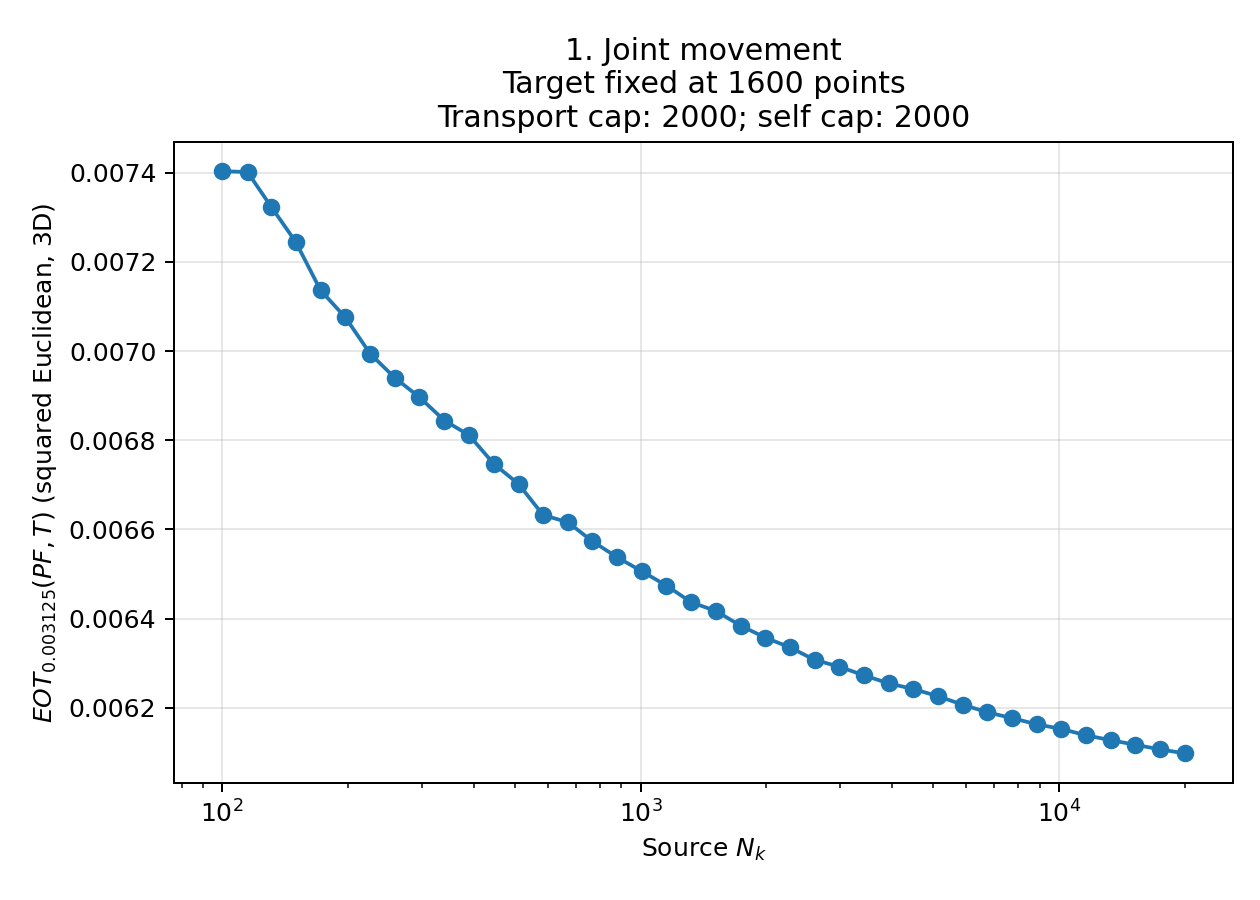
\includegraphics[width=0.88\textwidth]{high_iter_experiment_1.png}
 \caption{Experiment 1: joint movement of source count and refractor
 epsilon. Top: transport/self caps 17/17. Bottom: caps 2000/2000.
 Target fixed at 1600 points; evaluation epsilon fixed at 1/320.}
 \label{fig:new-experiment1}
\end{figure}
\begin{figure}[p]
 \centering
 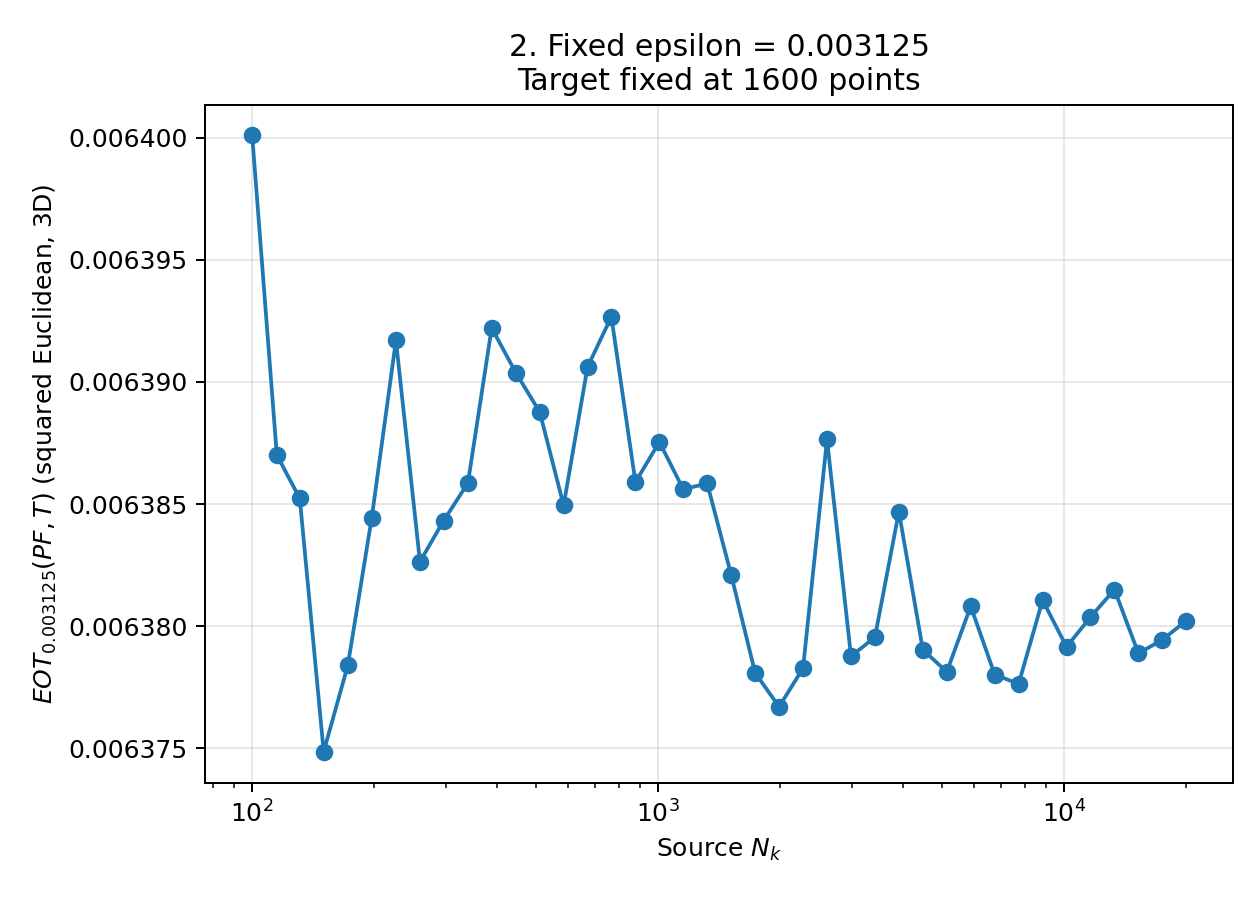
\includegraphics[width=0.88\textwidth]{baseline_experiment_2.png}
 \par\smallskip
 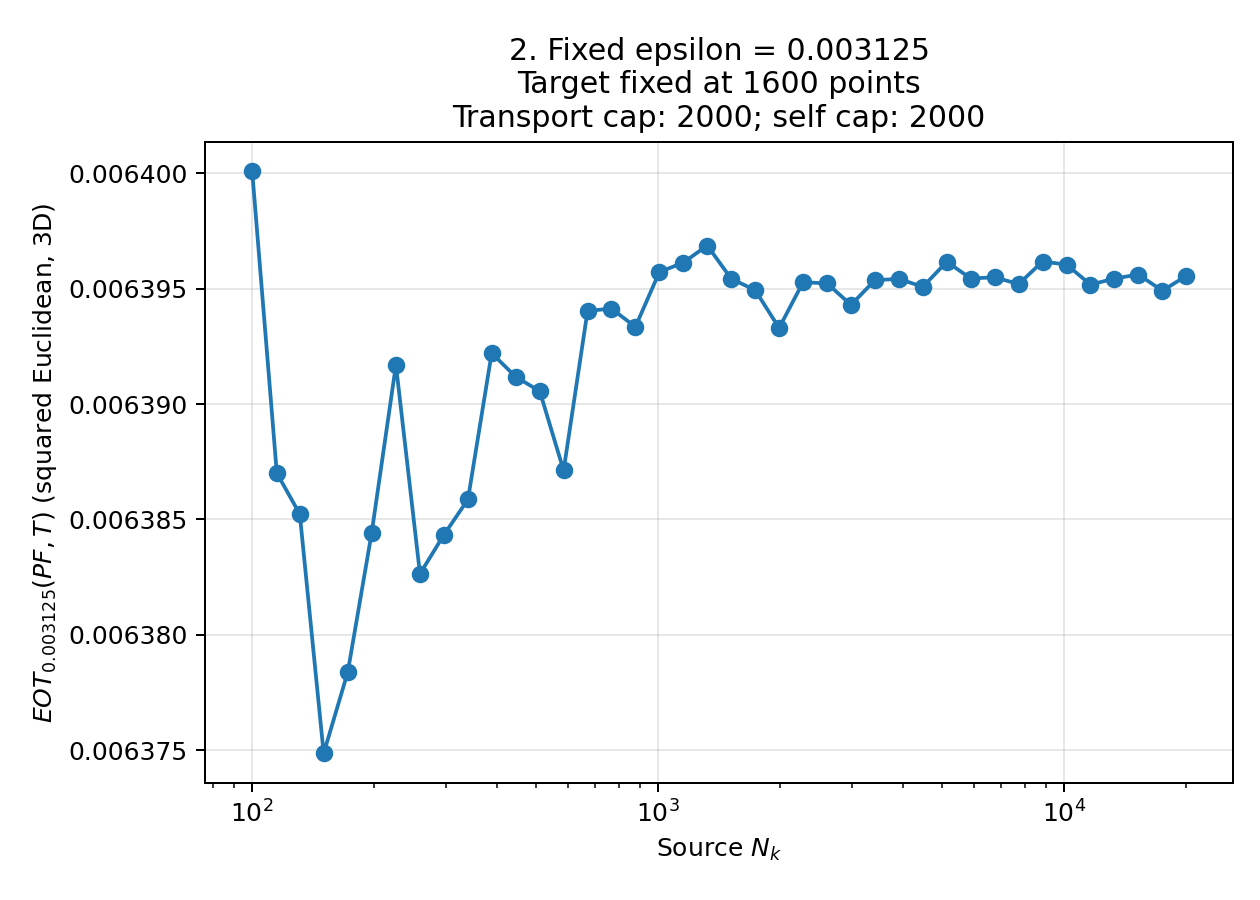
\includegraphics[width=0.88\textwidth]{high_iter_experiment_2.png}
 \caption{Experiment 2: source count varies, with refractor epsilon
 fixed at 1/320. Top: caps 17/17. Bottom: caps 2000/2000.
 Target fixed at 1600 points; evaluation epsilon fixed at 1/320.}
 \label{fig:new-experiment2}
\end{figure}
\begin{figure}[p]
 \centering
 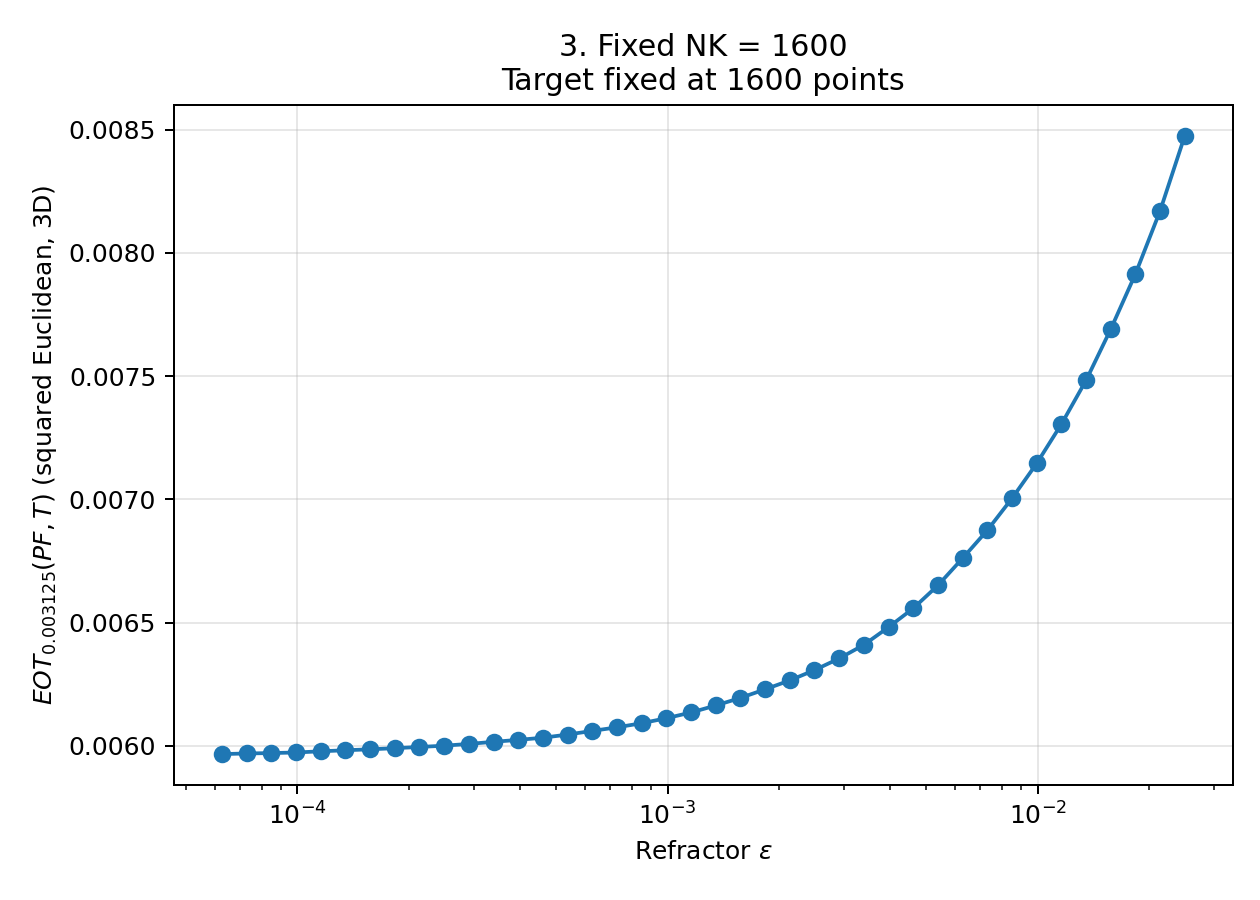
\includegraphics[width=0.88\textwidth]{baseline_experiment_3.png}
 \par\smallskip
 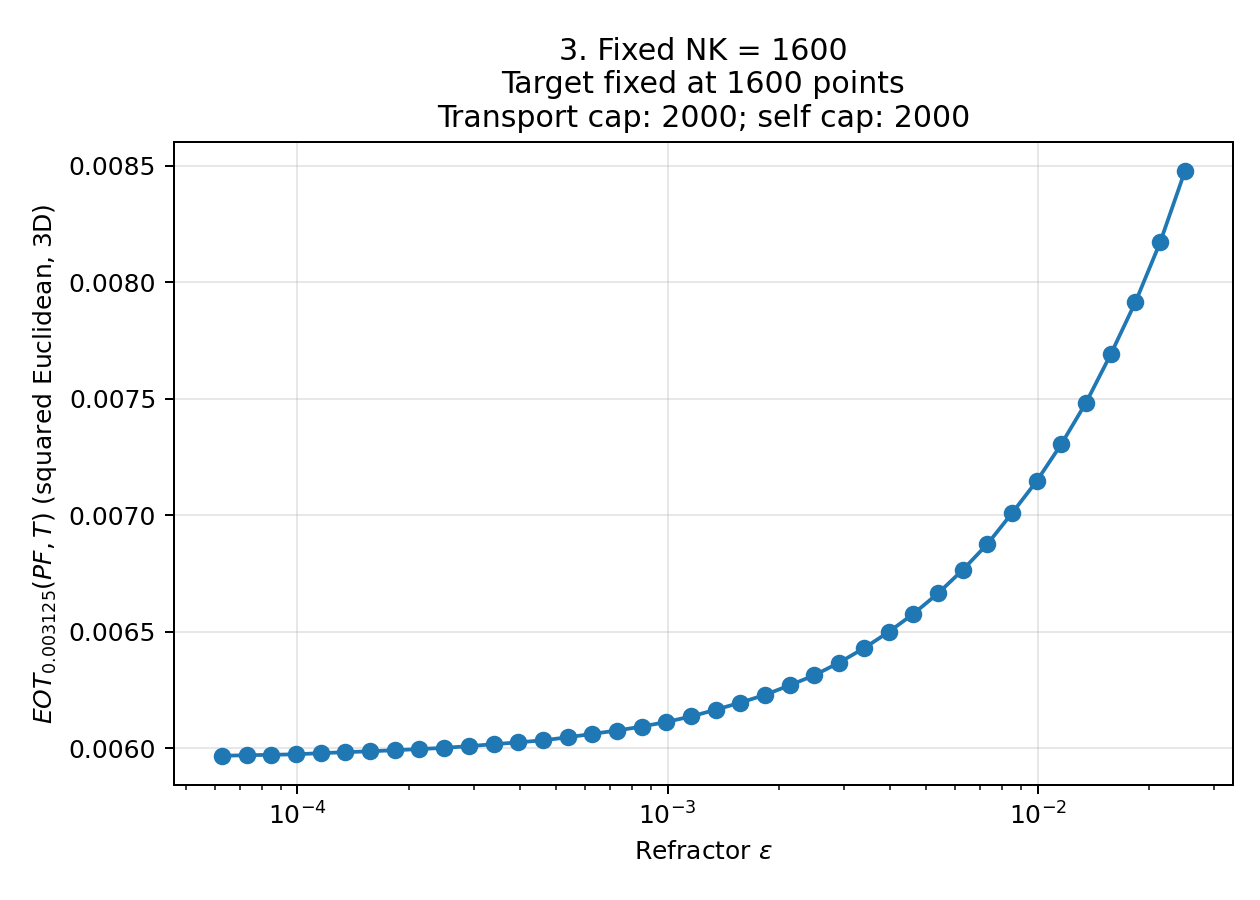
\includegraphics[width=0.88\textwidth]{high_iter_experiment_3.png}
 \caption{Experiment 3: refractor epsilon varies, with source count
 fixed at 1600. Top: caps 17/17. Bottom: caps 2000/2000.
 Target fixed at 1600 points; evaluation epsilon fixed at 1/320.}
 \label{fig:new-experiment3}
\end{figure}
\clearpage
